\section{Maximum Acceleration}

In this test we want to measure the maximum acceleration of our device. This lets us compare the limits of the different devices as well as the performance of the electronics (e.g. MIKE \#3 and MIKE \#6).

\subsection{Implementation}

In order to determine the maximum acceleration, the motor is fed with its maximum current for a short time. We want to know the positive as well as the negative maximum acceleration, this can be set in the frontend of the vi by selecting from cases "positive" and "negative". Keep in mind, that positive is a clockwise movement and negative is a counter-clockwise movement. The process can be started by pressing \emph{start}, however, before you do that you should move the end-effector to the end of its range of motion (i.e. for the clockwise movement, move the end effector to -90 degrees for the start).

\subsection{Data Analysis}

To determine the maximum acceleration, the measured position signal is recorded over time. The recorded signal is cut, so that only the measured points while the end-effector is moving are taken into account. This "shortened" signal is fitted with a polyfit in order to gain a time-dependant position function, which can then be derived two times in order to calculate the acceleration signal over time. The degree for the polyfit can be set in the code (try and error until it is just not over-fitted). The maximum acceleration can then be read from that signal. But one has to keep in mind that it is only an estimated signal, so it is advised to implement the measurement a few times and to compare the results.

\subsection{Results}

I did the measurements for MIKE \#6 and MIKE \#3. For each device I made three measurements for positive and negative acceleration. The results are shown in the following table.

\begin{table}[h]
\begin{tabular}{|l|ll|ll|}
\hline
                  & \multicolumn{2}{l|}{\textbf{MIKE 6}}                      & \multicolumn{2}{l|}{\textbf{MIKE 3}}                      \\ \hline
                  & \multicolumn{1}{l|}{\textbf{measurements [$\frac{rad}{s^2}$]}} & \textbf{avg [$\frac{rad}{s^2}$]} & \multicolumn{1}{l|}{\textbf{measurements [$\frac{rad}{s^2}$]}} & \textbf{avg [$\frac{rad}{s^2}$]} \\ \hline
                  & \multicolumn{1}{l|}{28'941}                &              & \multicolumn{1}{l|}{31'950}                 &              \\ \cline{2-2} \cline{4-4}
\textbf{positive} & \multicolumn{1}{l|}{23'995}                & 26'281        & \multicolumn{1}{l|}{27'145}                 & 31'439        \\ \cline{2-2} \cline{4-4}
                  & \multicolumn{1}{l|}{25'907}                &              & \multicolumn{1}{l|}{35'222}                 &              \\ \hline
                  & \multicolumn{1}{l|}{-28'042}                      &              & \multicolumn{1}{l|}{-33'013}                &              \\ \cline{2-2} \cline{4-4}
\textbf{negative} & \multicolumn{1}{l|}{-27'683}                      & -26'858             & \multicolumn{1}{l|}{-30'033}                & -32'280      \\ \cline{2-2} \cline{4-4}
                  & \multicolumn{1}{l|}{-24'850}                      &              & \multicolumn{1}{l|}{-33'795}                &              \\ \hline
\end{tabular}
\end{table}

It is visible that the maximum acceleration of MIKE \#3 is larger, this is due to the the fact that the new motor of MIKE \#6 provides less torque. What is strange though is that in the ICORR paper from 2019 \cite{icorr} a max acceleration of 52'000 $\frac{rad}{s^2}$, which is higher than the one I measured for MIKE \#3. A possible reason for that could be the different method used to derive the acceleration.\\

The following plot shows an example of the analysed position and velocity signals:

\begin{figure}[h]
 \centering
 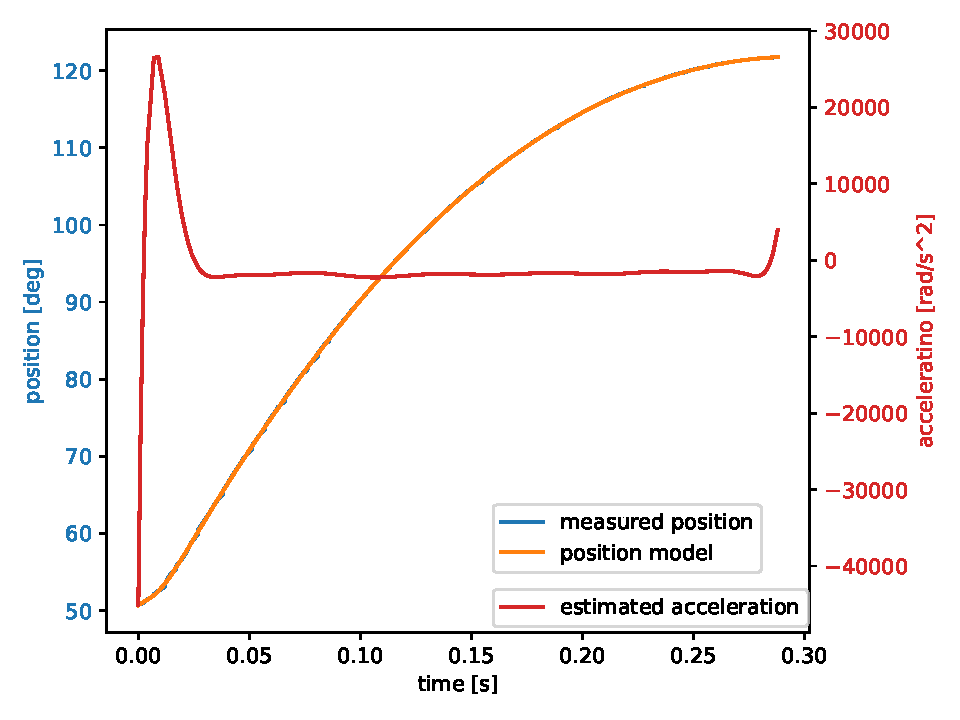
\includegraphics[width=0.8\textwidth]{chapters/maximum Acceleration/max_Acceleration_example.pdf}
 \caption{The plot shows the measurement of the maximum acceleration test of MIKE \#6. As one can see the model of the position fits the measurements.}
 \label{fig:meine-grafik}
\end{figure}